\documentclass[../../main.tex]{subfiles}

\begin{document}
\newpage
\subsubsection{Využitie IoT}
    Riešenie IoT sa môže implementovať pre široké spektrum aplikácií v rôznych odvetviach, ako je zdravotníctvo, služby, doprava, logistika, smart home, smart office...
    
    Podľa výskumu v Forrester Research \cite{Forrester} smart prostredie využíva informácie a komunikáciu na zefektívnenie a zinteraktívnenie komponentov kritickej infraštruktúry rôznych odvetví. V nasledujúcej tabuľke a na následnom obrázku sú vypísané a zobrazené domény možného využitia aplikácií pomocou riešenia  IoT.

% https://www.sciencedirect.com/science/article/pii/S0167739X13000241

\begin{table}[h!]
\centering
\begin{tabular}{|l|l|}
\hline
Smart domovy                                                              & \begin{tabular}[c]{@{}l@{}}ovládanie a bezpečnosť,inteligentná údržba,\\ ovládanie teploty, manažment energii,\\ rozpoznávanie tváre, biomedicína\end{tabular}                                     \\ \hline
Smart mestá                                                               & \begin{tabular}[c]{@{}l@{}}inteligentné monitorovanie, automatický transport,\\ presný manažment energie, environmentálne monitorovania\end{tabular}                                                                \\ \hline
Smart doprava                                                             & \begin{tabular}[c]{@{}l@{}}inteligentná kontrola premávky,\\ systém pre údržbu dopravných ciest,\\ systém parkovania, komunikácia RFID prvkami\end{tabular}                                             \\ \hline
\begin{tabular}[c]{@{}l@{}}Smart\\ maloobchod \\ a logistika\end{tabular} & \begin{tabular}[c]{@{}l@{}}riadenie dopravného reťazca, aplikácie nakupovania,\\ Smart manažment produktov, sledovanie zásob,\\ predajné terminály, predajné automaty\end{tabular}                   \\ \hline
\begin{tabular}[c]{@{}l@{}}Smart\\ Agrikultúra\end{tabular}               & \begin{tabular}[c]{@{}l@{}}senzory teploty a vlhkosti pôdy,\\ Smart zavlažovanie, Smart práškovanie\end{tabular}                                                                                      \\ \hline
\begin{tabular}[c]{@{}l@{}}Smart továrne \\ priemysel/biznis\end{tabular} & \begin{tabular}[c]{@{}l@{}}monitorovanie kvality vzduchu, monitorovanie teploty,\\ meranie ozónu v atmosfére,\\ vnútorná lokácia, autodiagnóza vozidla\\ senzori teploty a vlhkosti pôdy\end{tabular} \\ \hline
\begin{tabular}[c]{@{}l@{}}Smart zdravotná\\ starostlivosť\end{tabular}  & \begin{tabular}[c]{@{}l@{}}dohľad nad pacientom, športová starostlivosť,\\ ultrafialové žiarenie\end{tabular}                                                                                         \\ \hline
Smart oblečenie                                                           & \begin{tabular}[c]{@{}l@{}}Smart okuliare, Smart šaty, senzor spánku,\\ Smart hodinky\end{tabular}                                                                                                   \\ \hline
ostatné                                                                   & \begin{tabular}[c]{@{}l@{}}Smart múzeá, Smart školy, bankomaty\end{tabular}                                                                                                                         \\ \hline
\end{tabular}
\caption{\label{tab:table-name}Obor domén využitia IoT pre aplikácie}
\end{table}

\begin{figure}[h!]
    \centering
  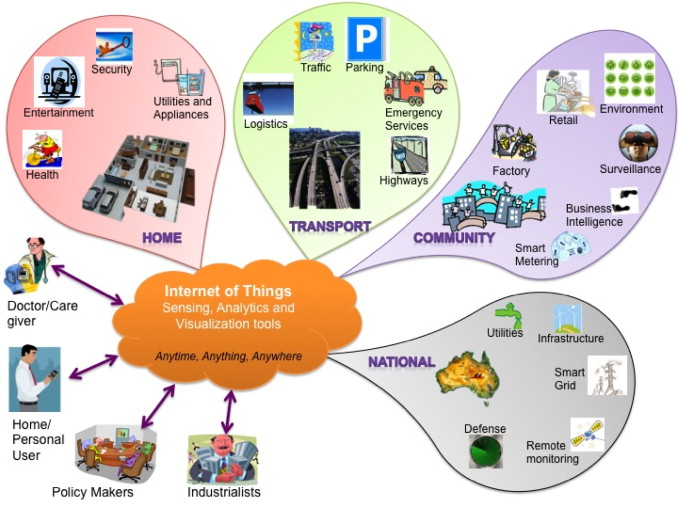
\includegraphics[scale=0.8]{images/IoT_domains.jpg}
  \caption{Schéma IoT\cite{GUBBI20131645}}
\end{figure} 
% \clearpage
\end{document}